% ===================================================================
\section{Gases: ideal, kinetic, equipartition, real}\label{sec:gases}
% ===================================================================
\begin{multicols}{2}
\subsection{Ideal-gas law in every basis}\label{sec:idealgas}
\CORE{}
\begin{formulabox}
\vspace{-6pt}
\begin{align}
PV &= nRT = NkT = mR_sT,\qquad R_s=R/M \label{F:gas:ideal}\\
\rho &= \frac{PM}{RT},\qquad P=\rho R_sT \label{F:gas:density}\\
\frac{P_1V_1}{n_1T_1} &= \frac{P_2V_2}{n_2T_2}\quad\text{(combined gas law)} \label{F:gas:combined}
\end{align}
\end{formulabox}
$P$ \textbf{absolute} (Pa), $T$ in K, $n$ in mol, $N$ molecules, $M$ in \si{kg/mol} when $R=\SI{8.314}{J/(mol.K)}$. $P_{\text{abs}}=P_{\text{gauge}}+P_{\text{atm}}$. For air $R_s=\SI{287.05}{J/(kg.K)}$ ($M=\SI{28.965}{g/mol}$).\src{CP} \textbf{$R$ in other units:} \tabinput{data/R_units.tex}\src{CODATA}

Special cases (hold the others fixed): Boyle $PV$ const ($n,T$); Charles $V/T$ const ($n,P$); Gay-Lussac $P/T$ const ($n,V$); Avogadro $V/n$ const ($T,P$).

\begin{reftab}{T:stp}{``Standard'' conditions are conventions---state which one.\src{DER}}
\small
\begin{tabularx}{\linewidth}{@{}Yccr@{}}
\toprule
Convention & $T$ & $P$ & $\bar V$ (\si{L/mol})\\
\midrule
IUPAC STP (since 1982) & \SI{273.15}{K} & \SI{100}{kPa} & 22.711\\
Older STP & \SI{273.15}{K} & \SI{101.325}{kPa} & 22.414\\
SATP & \SI{298.15}{K} & \SI{100}{kPa} & 24.790\\
\SI{25}{\celsius}, 1 atm & \SI{298.15}{K} & \SI{101.325}{kPa} & 24.465\\
``NTP'' (one usage) & \SI{293.15}{K} & \SI{101.325}{kPa} & 24.055\\
\bottomrule
\end{tabularx}\end{reftab}
Thermochemical standard state is $p^\circ=\SI{1}{bar}$ with \emph{no} fixed temperature (data usually at \SI{298.15}{K}).

\subsection{Mixtures: Dalton and mole fractions}\label{sec:dalton}
\begin{formulabox}
\vspace{-6pt}
\begin{align}
P &= \textstyle\sum_i p_i,\quad p_i=y_iP,\quad y_i=\frac{n_i}{n}=\frac{p_i}{P}=\frac{V_i}{V} \label{F:gas:dalton}\\
M_{\text{mix}} &= \textstyle\sum_i y_iM_i \label{F:gas:Mmix}
\end{align}
\end{formulabox}
$V_i$ = Amagat partial volume (component alone at mixture $T,P$). Mass fraction $w_i=y_iM_i/M_{\text{mix}}\ne y_i$. Dry air: $y\approx0.781$ \ce{N2}, 0.209 \ce{O2}, 0.0093 Ar, $\approx0.0004$ \ce{CO2} (rising).\src{EK} Gas over water: \eqp{F:phase:overwater}.

\begin{demobox}\textbf{Gas collected over water $\to$ molar mass.} \SI{250.0}{mL} of gas over water at \SI{22.0}{\celsius}, levels equalized, $P_{\text{atm}}=\SI{99.5}{kPa}$; dry-gas mass \SI{0.316}{g}. $p_{\text{sat}}(\SI{22}{\celsius})=\SI{2.645}{kPa}$,\src{IAPWS} so $p_{\text{gas}}=\SI{96.85}{kPa}$; $n=pV/RT=\SI{9.867}{mmol}$; $M=\SI{32.0}{g/mol}$ (\ce{O2}). Ignoring water vapor gives 31.2---a \SI{3}{\percent} error that can mis-identify the gas.\src{DER}\end{demobox}

\subsection{Kinetic theory and molecular speeds}\label{sec:kinetic}
\CORE{} Assumptions: many point-like molecules, random motion, elastic collisions, no forces except during collisions, Newtonian mechanics.
\begin{formulabox}
\vspace{-6pt}
\begin{align}
P &= \tfrac13\,n_N\,m\,\langle v^2\rangle,\qquad \langle \tfrac12 mv^2\rangle=\tfrac32kT \label{F:gas:kinetic}\\
v_{\text{rms}} &= \sqrt{\frac{3RT}{M}},\ \ \bar v=\sqrt{\frac{8RT}{\pi M}},\ \ v_{\text{mp}}=\sqrt{\frac{2RT}{M}} \label{F:gas:speeds}\\
f(v) &= 4\pi\Big(\frac{m}{2\pi kT}\Big)^{3/2}v^2\,e^{-mv^2/2kT} \label{F:gas:maxwell}
\end{align}
\end{formulabox}
$n_N=N/V$ (number density, \si{m^{-3}}), $m=M/N_A$ (kg per molecule). Ratios $v_{\text{mp}}:\bar v:v_{\text{rms}}=1:1.128:1.225$. \textbf{$M$ in kg/mol} (\SI{0.028}{kg/mol} for \ce{N2}, not 28).

\textbf{Speed vs velocity.} Each velocity component is Gaussian with mean zero, $\langle v_x^2\rangle=kT/m$; the average \emph{velocity} of a gas at rest is zero, while the average \emph{speed} $\bar v>0$. $f(v)$ is normalized: $\int_0^\infty f\,\dd v=1$; units \si{s/m}.

\begin{reffig}{fig:maxwell}{Maxwell speed distribution for \ce{N2}, computed from \eqref{F:gas:maxwell} (each curve has unit area, checked numerically).\src{DER} Hotter gas: peak moves right and drops.}
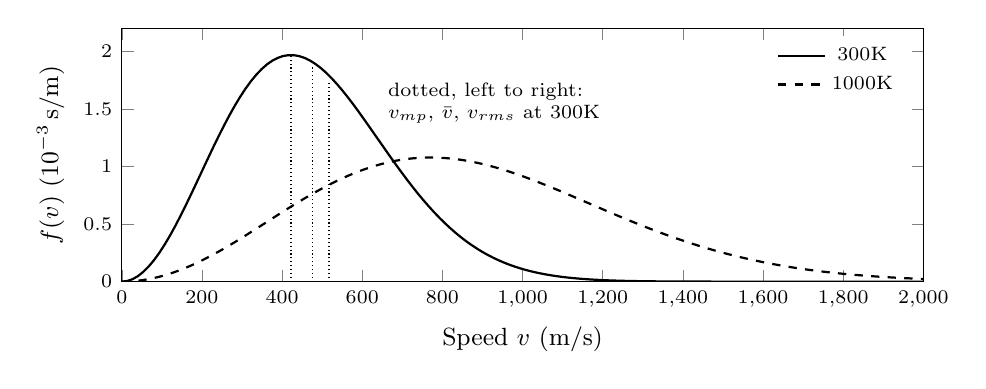
\begin{tikzpicture}
\begin{axis}[width=0.97\linewidth,height=4.8cm,xmin=0,xmax=2000,ymin=0,ymax=2.2,
  xlabel={Speed $v$ (\si{m/s})},ylabel={$f(v)$ ($10^{-3}$\,\si{s/m})},
  tick label style={font=\scriptsize},label style={font=\small},samples=150,domain=0:2000,
  legend style={font=\scriptsize,draw=none,at={(0.98,0.97)},anchor=north east},scaled x ticks=false]
\addplot[thick,black] {1000*4*pi*(0.0280134/(2*pi*8.314462618*300))^1.5*x^2*exp(-0.0280134*x^2/(2*8.314462618*300))};
\addlegendentry{\SI{300}{K}}
\addplot[thick,black,dashed] {1000*4*pi*(0.0280134/(2*pi*8.314462618*1000))^1.5*x^2*exp(-0.0280134*x^2/(2*8.314462618*1000))};
\addlegendentry{\SI{1000}{K}}
\draw[densely dotted] (axis cs:422,0)--(axis cs:422,1.97);
\draw[densely dotted] (axis cs:476.2,0)--(axis cs:476.2,1.87);
\draw[densely dotted] (axis cs:516.8,0)--(axis cs:516.8,1.74);
\node[font=\scriptsize,anchor=west,align=left] at (axis cs:640,1.55) {dotted, left to right:\\$v_{\text{mp}}$, $\bar v$, $v_{\text{rms}}$ at \SI{300}{K}};
\end{axis}
\end{tikzpicture}
\end{reffig}

\begin{demobox}\textbf{\ce{N2} at \SI{300}{K}, 1~atm.} $v_{\text{mp}}=\SI{422}{m/s}$, $\bar v=\SI{476}{m/s}$, $v_{\text{rms}}=\SI{517}{m/s}$ (numerical moments of $f(v)$ agree). With collision diameter $d\approx\SI{0.37}{nm}$ (approximate), $n_N=P/kT=\SI{2.45e25}{m^{-3}}$, mean free path $\lambda=\SI{67}{nm}$, collision frequency $z=\bar v/\lambda=\SI{7.1e9}{s^{-1}}$.\src{DER}\end{demobox}

\subsection{Effusion, diffusion, mean free path}\label{sec:effusion}
\begin{formulabox}
\vspace{-6pt}
\begin{align}
\Phi &= \tfrac14\,n_N\,\bar v\quad\text{(molecules per area per time)} \label{F:gas:effusion}\\
\frac{\text{rate}_1}{\text{rate}_2} &= \sqrt{\frac{M_2}{M_1}}\quad\text{(Graham)} \label{F:gas:graham}\\
\lambda &= \frac{1}{\sqrt2\,\pi d^2 n_N}=\frac{kT}{\sqrt2\,\pi d^2P} \label{F:gas:mfp}
\end{align}
\end{formulabox}
\textbf{Effusion} = escape through a hole small compared with $\lambda$ (no collective flow). Graham's ratio requires the \emph{same} $T$, same number density (pressure), and the same hole; the time to effuse equal amounts scales as $\sqrt M$. \textbf{Diffusion} = interpenetration through collisions; it depends on molecular size and the partner gas, so Graham's law is only a rough guide (hard-sphere estimate $D\sim\tfrac13\lambda\bar v$).\src{EK}

\textbf{Example:} \ce{H2} vs \ce{O2} through the same pinhole at the same $T$ and $P$: rate ratio $\sqrt{32.00/2.016}=3.98$; \ce{O2} takes $3.98\times$ as long to lose the same number of moles.\src{DER}

\textbf{Density trap:} $n_N$ in \eqref{F:gas:mfp} is \emph{number} density (\si{m^{-3}}), not molar density (\si{mol/m^3}); $n_N=N_A\,(n/V)$.

\subsection{Equipartition and heat capacities}\label{sec:equipartition}
\CORE{} Classically, each \emph{active} quadratic energy term contributes $\tfrac12kT$ per molecule ($\tfrac12RT$ per mole). A fully active vibrational mode contributes two terms (kinetic + potential), i.e.\ $R$ per mole.
\begin{formulabox}
\vspace{-6pt}
\begin{align}
\bar C_p-\bar C_v &= R\ \ \text{(molar)};\quad C_p-C_v=nR;\quad c_p-c_v=R_s \label{F:gas:mayer}\\
\gamma &= \bar C_p/\bar C_v \label{F:gas:gamma}
\end{align}
\end{formulabox}
\begin{reftab}{T:equipartition}{Rigid-molecule (vibration frozen) equipartition predictions.\src{EK}}
\small
\begin{tabularx}{\linewidth}{@{}Ycccc@{}}
\toprule
Molecule & dof (tr+rot) & $\bar C_v/R$ & $\bar C_p/R$ & $\gamma$\\
\midrule
Monatomic (He, Ar) & 3+0 & 1.5 & 2.5 & 5/3\\
Linear (\ce{N2}, \ce{O2}, \ce{CO2}) & 3+2 & 2.5 & 3.5 & 7/5\\
Nonlinear (\ce{H2O}, \ce{CH4}) & 3+3 & 3.0 & 4.0 & 4/3\\
\bottomrule
\end{tabularx}\end{reftab}
Vibrational modes: $3N_a-5$ (linear), $3N_a-6$ (nonlinear) for $N_a$ atoms. \textbf{Freeze-out:} quantum level spacing larger than $kT$ makes a mode inactive. At \SI{300}{K}, \ce{N2}/\ce{O2} vibration is essentially frozen ($\bar C_p/R=3.51$, 3.54), while \ce{CO2} is \emph{between} rigid (3.5) and fully excited (7.5) at 4.51 because its low-frequency bending modes are partly active (\tref{T:gases300}).\src{CP} So ``$\gamma=1.4$'' is an idealization that drifts with temperature. Solids: 3 kinetic + 3 potential terms give $3R$ (Dulong--Petit).
\end{multicols}

\begin{reftab}{T:gases300}{Gas properties at \SI{300}{K}, \SI{100}{kPa} from reference equations of state and transport models.\src{CP} $^\ast$Steam row at \SI{400}{K} (water is liquid at \SI{300}{K}, \SI{100}{kPa}).}
\small
\begin{tabularx}{\textwidth}{@{}lYYYYYYY@{}}
\toprule
Gas & $M$ & $c_p$ & $\bar C_p/R$ & $\gamma$ & $k$ & $\mu$ & $Z$\\
 & (\si{g/mol}) & (\si{J/(kg.K)}) & & & (\si{mW/(m.K)}) & (\si{\micro Pa.s}) & \\
\midrule
\tabinput{data/gases_300K.tex}
\bottomrule
\end{tabularx}\end{reftab}

\begin{multicols}{2}
\subsection{Real gases}\label{sec:realgas}
\CORE{} \textbf{Compressibility factor} $Z=P\bar V/(RT)$; $Z=1$ ideal. $Z<1$: attractions dominate (moderate $P$, lower $T$); $Z>1$: excluded volume dominates (high $P$). Examples: \ce{CO2} at \SI{300}{K}: $Z=0.995$ at \SI{0.1}{MPa}, 0.687 at \SI{5}{MPa}; \ce{N2} at \SI{300}{K}: 1.005 at \SI{10}{MPa}, 1.364 at \SI{50}{MPa}.\src{CP}
\begin{formulabox}van der Waals ($\bar V=V/n$):
\begin{equation}
\Big(P+\frac{a}{\bar V^2}\Big)(\bar V-b)=RT \label{F:gas:vdw}
\end{equation}
\vspace{-12pt}
\begin{align}
\bar V_c&=3b,\quad T_c=\frac{8a}{27Rb},\quad P_c=\frac{a}{27b^2},\quad Z_c=\tfrac38 \label{F:gas:vdwcrit}\\
a&=\frac{27R^2T_c^2}{64P_c},\qquad b=\frac{RT_c}{8P_c} \label{F:gas:vdwab}
\end{align}
\end{formulabox}
$a$: attraction (reduces wall pressure); $b$: excluded volume per mole. Units: $a$ in \si{Pa.m^6/mol^2} ($1=10$\,\si{L^2.bar/mol^2}); $b$ in \si{m^3/mol} ($10^{-3}$\,\si{m^3/mol} $=1$\,\si{L/mol}). Domain $\bar V>b$. Critical relations verified symbolically ($\partial P/\partial\bar V=\partial^2P/\partial\bar V^2=0$).\src{DER} Real $Z_c$ values are 0.23--0.30 (\ce{H2O} 0.229, \ce{CO2} 0.275, \ce{N2} 0.289),\src{CP} so vdW is qualitative near the critical point.

\begin{reftab}{T:vdw}{van der Waals constants fitted to each gas's critical point.\src{CP}\src{DER} Textbook tables fitted differently can disagree by a few percent.}
\small
\begin{tabularx}{\linewidth}{@{}lYYYY@{}}
\toprule
Gas & $T_c$ & $P_c$ & $a$ & $b$\\
 & (K) & (MPa) & (\si{L^2.bar/mol^2}) & (\si{L/mol})\\
\midrule
\tabinput{data/vdw.tex}
\bottomrule
\end{tabularx}\end{reftab}

\begin{demobox}\textbf{How good is van der Waals?} \ce{CO2} at \SI{300}{K}, \SI{5.0}{MPa}. Ideal gas: $\bar V=RT/P=\SI{0.499}{L/mol}$. vdW with \tref{T:vdw} constants (cubic in $\bar V$; one real root here): $\bar V=\SI{0.365}{L/mol}$, $Z=0.731$. Reference equation of state: $Z=0.687$.\src{CP} vdW captures most of the deviation (ideal: $Z=1$) but not all; near the critical point it is only qualitative.\src{DER}\end{demobox}

\textbf{Virial form} (extension): $Z=1+B(T)/\bar V+C(T)/\bar V^2+\dots$; vdW gives $B=b-a/(RT)$, so the \textbf{Boyle temperature} (where $B=0$) is $T_B=a/(Rb)$.\src{DER} \EXT

\begin{trapbox}An equation of state alone gives $P$--$\bar V$--$T$, not $c_p$, $h$, or $s$; caloric properties need ideal-gas heat capacities plus departure terms (or tables). For a vdW gas $U=nC_vT-an^2/V$, so even free expansion cools it slightly; an ideal gas does not cool.\src{DER}\end{trapbox}
\end{multicols}
